\let\textcircled=\pgftextcircled
\chapter{Algorithms}
\renewcommand{\ttdefault}{pcr}
\lstset{
	basicstyle=\small\ttfamily,
	captionpos=t,
	numbers=left,
	tabsize=4,
	keywordstyle=\bfseries,
	breaklines=true,
	columns=fullflexible,
	numbersep=-8pt, 
	frame = shadowbox,
	morekeywords={BEGIN, END, DISPLAY, INPUT, IF, ENDIF, WHILE, DO, ELSE, THEN, OR, OPEN, RETURN, WRITE, NEXT, FOR, APPEND, CLOSE, PASS, AND, OUTPUT}
}

\section{Information Surrounding Blockchain Development}

This section will explain concepts that are fundamental to blockchain development and will give an insight into how all the different parts work together to create a functioning network.

The runtime of a blockchain is the business logic that defines its behaviour. In Substrate-based chains, the runtime is referred to as the "state transition function"; it is where Substrate developers define the storage items that are used to represent the blockchain's state as well as the functions that allow blockchain users to make changes to this state. Thus, the runtime can simply be thought of as the business logic of the chain. It defines what transactions are valid and invalid and determines how the chain's state changes in response to transactions.\\

The "outer node", everything other than the runtime, does not compile to WASM, only to native. The outer node is responsible for handling peer discovery, transaction pooling, block and transaction gossiping, consensus, and answering RPC calls from the outside world. While performing these tasks, the outer node sometimes needs to query the runtime for information or provide information to the runtime. A Runtime API facilitates this kind of communication between the outer node and the runtime. \\

An extrinsic is a piece of information that comes from outside the chain and is included in a block. Extrinsics fall into three categories: inherents, signed transactions, and unsigned transactions. A block in Substrate is composed of a header and an array of extrinsics. The header contains a block height, parent hash, extrinsics root, state root, and digest.  Extrinsics are bundled together into a block as a series to be executed as each is defined in the runtime. \\

Blockchains must agree on:

\begin{itemize}
	\item Some initial state, called "genesis", 
	\item A series of state transitions, each called a "block", and
	\item A final (current) state.
\end{itemize}

In decentralized systems, the nodes will see transactions in different orders, and thus they must use elaborate method to exclude transactions. As a further complication, blockchain networks strive to be fault tolerant, which means that they should continue to provide consistent data even if some participants are not following the rules. \\

Blockchain nodes use consensus engines to agree on the blockchain's state. It has some internal state, and state transition function that allows it to transition from its current state to a future state. In most runtimes there are states that have valid transitions to multiple future states, but a single transition must be selected. \\

Some nodes in a blockchain network are able to produce new blocks, a process known as authoring. This is decided by the consensus engine that is being used. For this permissoned blockchain, the consensus method that will be used is Aura (round-robin). Aura provides a slot-based block authoring mechanism where a known set of authorities take turns producing blocks. Further, a fork choice rule is an algorithm that takes a blockchain and selects the "best" chain, and thus the one that should be extended. The longest chain rule simply says that the best chain is the longest chain. \\

Users in any system want to know when their transactions are finalized, and blockchain is no different. In some traditional systems, finality happens when a receipt is handed over, or papers are signed. Using the block authoring schemes and fork choice rules described so far, transactions are never entirely finalized. There is always a chance that a longer (or heavier) chain will come along and revert your transaction. However, the more blocks are built on top of a particular block, the less likely it is to ever be reverted. In this way, block authoring along with a proper fork choice rule provides probabilistic finality. When deterministic finality is desired, a finality gadget can be added to the blockchain's logic. Members of a fixed authority set cast finality votes, and when enough votes have been cast for a certain block, the block is deemed final. In this system, this threshold is 2/3. Blocks that have been finalized by such a gadget cannot be reverted without external coordination such as a hard fork. The gadget that will be used is GRANDPA or GHOST-based Recursive Ancestor Deriving Prefix Agreement.
GRANDPA validators vote on chains, not blocks, i.e. they vote on a block that they consider "best" and their votes are applied transitively to all previous blocks. Once more than 2/3 of the GRANDPA authorities have voted for a particular block, it is considered final. A diagram of this process is below:\\

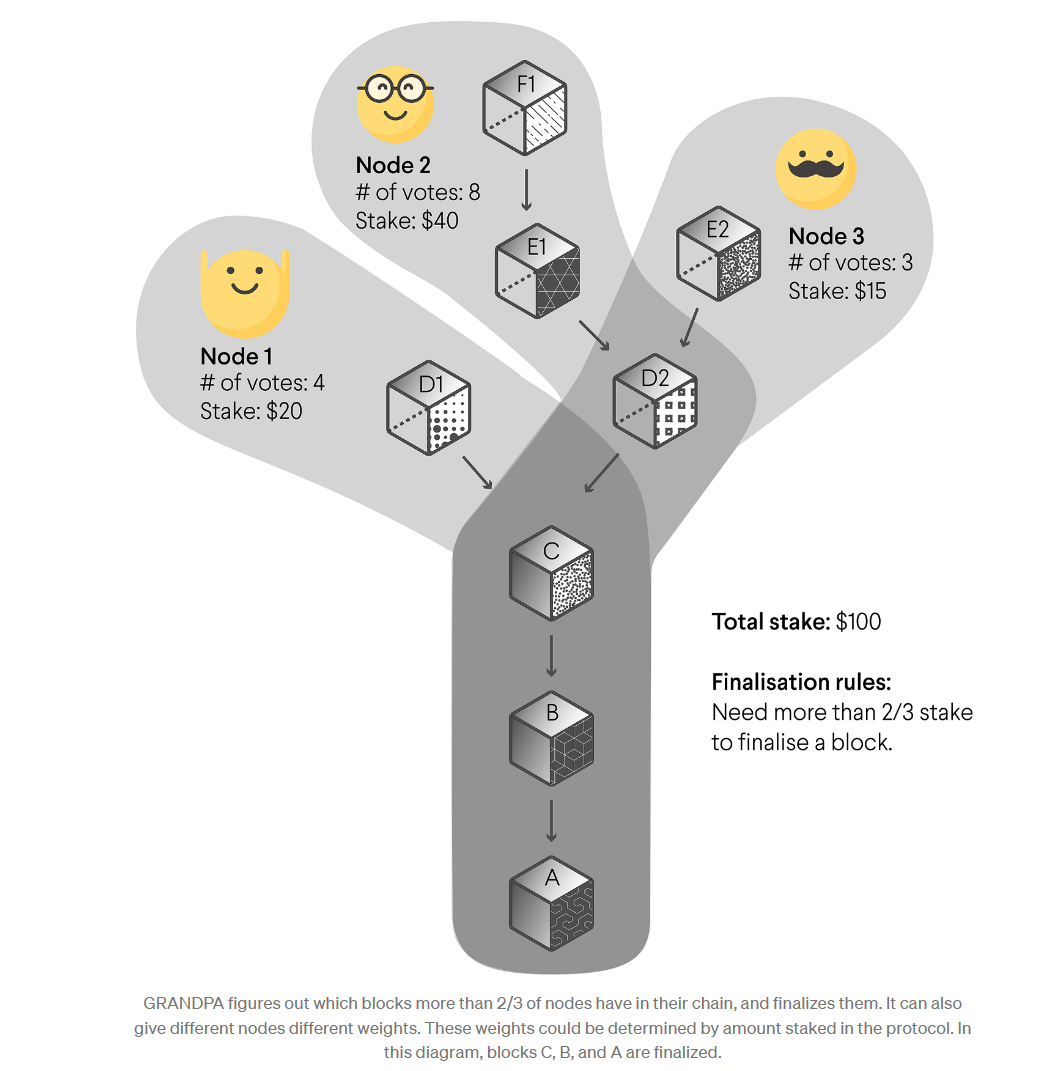
\includegraphics[width=\linewidth]{figures/finality.png} \\

Functions can be automated through smart contracts, in which lines of computer code use data from the blockchain to verify when contractual obligations have been met and payments can be issued. Smart contracts can be programmed to assess the status of a transaction and automatically take actions such as releasing a payment, recording ledger entries, and flagging exceptions in need of manual intervention. \\

Finally, a common architecture pattern for privacy-preserving is to only store a hash of the transaction data. For example, an invoice can be shared without exposing any details of the invoice. This allows companies to trace and exchange information with blockchain technology without exposing any data as the data are kept safely off-chain. \\


The core algorithms that will be used in the application are displayed below, written in the pseudo-code syntax. The program is split into two sections: the node that will be apart of the network, and the front-end that will be accessed by business's and clients after they have set up the node. \\

\section{Algorithms - Node}
\subsection{Node Main Program}

\begin{lstlisting}[caption=Main Program, escapechar=\@]
	BEGIN MAINPROGRAM(node_key, port, ws_port, rpc_port, ed25519_key, sr25519_key, bootnodes)

non_fungible_Tokens()
runtime()

\end{lstlisting}

\subsection{Runtime}

\begin{lstlisting}[caption=Update User Data, escapechar=\@]
	BEGIN  @\underline{UpdateUserData(dataID, username, data)}@
		OPEN UserDatabase for relative access
		dataIDs = array of identifiers of all questions // These should correlate to dataID passed into function when retrieving the user preferences.
		FOR i=0 to users.len() DO
			IF users[i].username == username THEN
				FOR i=0 to dataIDs.len() DO
					IF dataIDs[i] == dataID THEN
						WRITE UserData.users[i] from data using dataID	
					ENDIF
				NEXT i
			ENDIF
		NEXT i
		CLOSE UserDatabase
	END  @\underline{UpdateUserData}@
\end{lstlisting}
\subsection{Non-fungible Tokens}

\section{Algorithms - Front-end}

\subsection{Main Program}

\begin{lstlisting}[caption=Machine Learning Recommendations and Optimisation, escapechar=\@]
	BEGIN  @\underline{MachineLearningRecomendations(ml\_input\_data)}@
		business_records, user_data, budget, from, to, duration, group_size, transport_data = ml_input_data // Data that the machine learning model will use to make sophisticated decisions about events to recommend the user. This is decompressing the tuple into multiple variables for utilisation.
		FOR i=0 to user_data.len() DO
			FOR j=0 to business_records.events.len() DO
				similarity_matrix[i][j] = cosine_similarity(user_data[i], budget, business_records.events[i]) // Constructs the similarity matrix based upon the similarity of user preferences and target budget with the different events.
			NEXT j
		NEXT i

		bayesian_network = @\underline{BayesianGeneration(similarity\_matrix, transport\_data)}@ //Transport data is used in the Bayesian network generation to link events not only by similarity and budget, but also the ability to be transported between the different locations.

		availabilities = business_records.availability
		recommendations = @\underline{GradientDescentOptimisation(availabilities,}@ @\underline{duration, user\_data, bayesian\_network)}@ //Optimisation of the timing of each event to make sure that the Itinerary lines up. Works by making steps towards a perfectly fitted timeslot by moving towards a minima and evaluating its performance based on a reward function. Utilises the events that are linked with the highest weighted similarity on the Bayesian network. 

		RETURN recommendation // Data type of recommendation is an event from business_records.events
		

	END  @\underline{MachineLearningRecomendations(ml\_input\_data)}@
			
\end{lstlisting}
\subsection{Display Non-fungible Tokens Module}

\begin{lstlisting}[caption= Interaction with Transport APIs, escapechar=\@]
	BEGIN  @\underline{TransportAPI(duration)}@
		transport_services = multidimensional array of n elements of [transportID, api_key, query_address] // All the api_keys needed to access the APIs of different transportation APIs, the multidimensional array of 3 by n, is so that each api key is coupled with a transport ID and query address so that each transport service can be identified and queried.

		transport_data = empty multidimensional array // This array will contain each transport and the times of arrival and location for each transport service.
		FOR i=0 to transport_services.len() DO
			transport_data[i] = @\underline{HttpRequest(transport\_services[i][0],}@ @\underline{transport\_services[i][1], transport\_services[i][2])}@ 
		NEXT i
		RETURN transport_data
	END  @\underline{TransportAPI}@
\end{lstlisting}


\vfill{}
